\documentclass[conference, 12pt, a4paper]{IEEEtran}
\usepackage[T1]{fontenc}
\usepackage[utf8]{inputenc}
\usepackage{url}
%\usepackage{underscore}
\usepackage{graphicx}
\usepackage{caption, subcaption}
\usepackage{geometry}
\usepackage{cite}
\usepackage{amsmath,amssymb,amsfonts}
\usepackage{textcomp}
\usepackage{xcolor}

%\def\BibTeX{{\rm B\kern-.05em{\sc i\kern-.025em b}\kern-.08em
%    T\kern-.1667em\lower.7ex\hbox{E}\kern-.125emX}}

\begin{document}

\title{DIRTY COW GÜVENLİK AÇIĞI}
\author{BAYRAM YARIM - 18010011067}

\maketitle
\begin{sloppypar}
\begin{abstract}
    \title\textbf{ÖZET}\\
    Açık kaynak kodlu yazılım geliştirme alanında lider olan şirket Red Hat, 2016 yılında Linux Kernelinde oldukça ciddi bir hatayla karşılaştığını duyurdu. Bahsi geçen hata \textbf{Dirty COW (CVE-2016-5195)} olarak adlandırıldı. Dirty Cow adının verilmesinin sebebi, Linux Kernel mekanizmasında bulunan \textbf{copy-on-write (COW)}. Hata \textbf{‘çok tehlikeli’} çünkü bu hata sayesinde saldırgan salt okunur belleğe/dosyaya yazma erişimi vermesine yarıyor.

    Herhangi bir saldırgan sistemin salt okunur dosyalarına yazma erişimi sağlayarak hatadan faydalanabilir. Azimuth Security firmasının kıdemli güvenlik araştırmacılarından Dan Rosenberg, bulunan bu hatanın Linux sistemlerinde şimdiye kadar bulunmuş en tehlikeli hata olduğunu açıkladı. Dirty Cow aynı zamanda shell erişimi sağlayan Web Hosting servis sağlayıcılarına karşı da kullanılabilir. Böyle bir hizmet sağlayıcının biri SQL injection ile Dirty Cow’un birleşimi sayesinde root erişimine sahip olabilir. Linux bu hata ortaya çıktıktan hemen sonra düzeltmek için bir güncelleme yayınladı ve Linux kullanan herkesin güncellemeyi acilen yapmaları gerektiği konusunda kullanıcılarını uyardı.[1]

    Çalışmalar için öncelikle sisteme Ubuntu 12.04 versiyonu kurulumu gerçekleştirildi. Ubuntu üzerinde linux kernelinin 3.11.0 versiyonu bulunmaktadır. Uygulama sadece kernel versiyonu 2.6.22 - 4.8.3 arasında olan tüm linux tabanlı işletim sistemlerinde/cihazlarda uygulanabilir. Örnek uygulamanın kod dosyasını indirdim ve kendime göre uyarlamaya başladım. Örneği uygulamak için öncelikle sistem üzerinde salt-okunur(izin modu 0644) bir dosya oluşturuldu ve içerisine değiştirilmesi için bir metin eklendi. Kod dosyasını derledim ve ilgili dosyaya erişim sağlayarak içeriğini değiştirme işlemini gerçekleştirdim.
\end{abstract}

%\section{Özet(Abstract)}

\section{Giriş (Introduction)}
    Açık kaynak kodlu yazılım geliştirme alanında lider olan şirket Red Hat, 2016 yılında Linux kernelinde oldukça ciddi bir hatayla karşılaştığını duyurdu. Bahsi geçen hata \textbf{Dirty COW (CVE-2016-5195)} olarak adlandırıldı. Dirty Cow adının verilmesinin sebebi, Linux Kernel mekanizmasında bulunan \textbf{copy-on-write (COW)}. Hata \textbf{‘çok tehlikeli’} çünkü bu hata sayesinde saldırgan salt okunur belleğe/dosyaya yazma erişimi vermesine yarıyor.

    Bu çalışmanın konusu Dirty COW güvenlik açığını amacı Dirty COW açığından yararlanarak salt okunur bir dosyaya erişim sağlayarak yazma işlemini gerçekleştirmektir. 

\section{Literatur Taraması (Literature Review)}
    %Bu bölüme çalışmanın konusuyla ilgili güncel literatür taramasına yer verilmelidir.
    Literatur taraması sonucu DirtyCOW açığının bir çok uygulaması vardır. Uygulamalar ile bu açıktan yararlanılarak linux tabanlı işletim sistemlerine / android cihazlara ve daha bir çok sisteme saldırı yapılabilmektedir. Fakat bu güvenlik açığı 2017 yılında tamamen kapatılmıştır. Her ne kadar bu güvenlik açığı tamamen kapatılsa da bazı sebeplerden dolayı sistem(kernel) güncellemesi yapılmayan cihazlar/işletim sistemleri halen bulunmaktadır. Mevcut bu durum saldırganlar için halen cazip bir alandır.

    Bu uygulamalar ile linux tabanlı işletim sistemlerinde normal kullanıcılara root yetkisi verilebilmektedir. Kütüphane dosyaları, dosya içerikleri değiştirilebilmektedir. Web sunucularına sql injection ile saldırı yapıp sunucu tamamen ele geçirilebilir. Sistem kütüphanelerine exploitler eklenebilir. Bu saldıralara benzer bir çok daha saldırı bu açıklıktan yararlanarak yapılabilir. Bu güvenlik açığı şu ana kadar linux kernelinde bulunan en yüksek ve tehlikeli bir durumdur. Güncel bu tarama sonucu linux kernel versiyonu eski olan (2.6.22 ile 4.8.3 arası) tüm sistemler güncellenmelidir. 

\section{Yöntem (Methodology)}
    Yöntem olarak bu açıktan yararlanarak hafıza birimi üzerinden dosyaya erişim sağlayarak dosya içeriğini değiştirmeyi örnek olarak yaptım.
    Öncelikle bu açığın uygulamasını yapmak için Ubuntu 12.04 versiyonunu VirtualBox üzerine kurulumunu gerçekleştirdim. Ubuntu 12.04 üzerinde kernel olarak 2014 yılında derlenmiş \textbf{3.11.0} versiyonu vardır. 
     
    \begin{figure}[htbp]
        \centering
        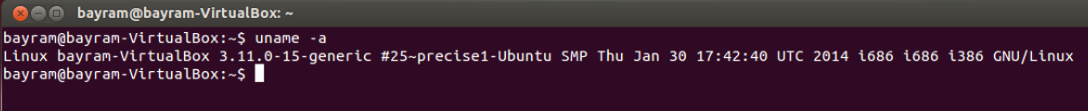
\includegraphics[scale=0.40]{ubuntu-os-info.png}
        \caption{Ubuntu Kernel Version}
    \end{figure}
    
    Daha sonra SeedLabs üzerinde bulunan örnek kod dosyasını indirdim ve kendime göre uyarlamaya başladım. Örneği uygulamak için öncelikle sistem üzerinde salt-okunur(0644) bir dosya oluşturdum ve içerisine bir yazı yazdım. Daha sonra dosya üzerinde işlem yapmak istediğimde \textbf{Permission Denied} uyarısı aldım. Aşağıdaki resimde yaptığım aşamaların ekran görüntüsü.
    \begin{figure}[htbp]
        \centering
        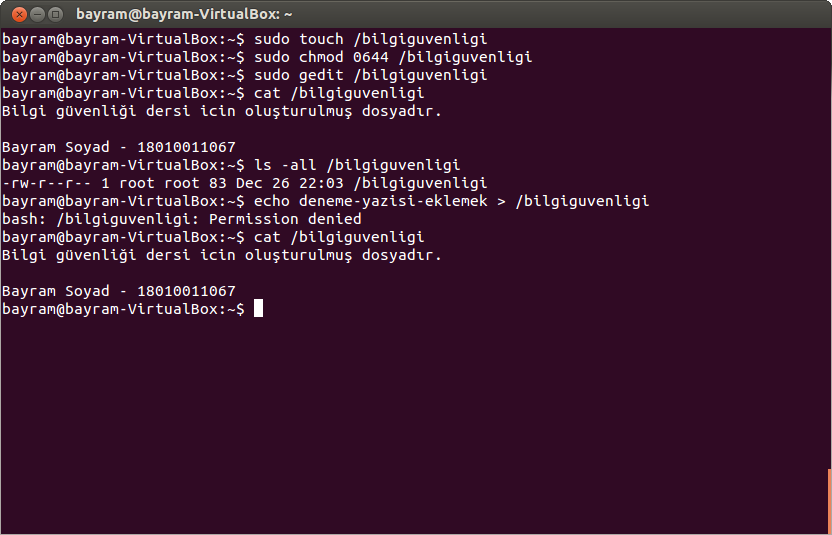
\includegraphics[scale=0.25]{process1.png}
        \caption{Dosya İşlemleri}
        %\label{fig:label}
    \end{figure}

    Bu işlemleri hallettikten sonra örnek kodu kendime göre uyarladım ve dosya içerisine yazmış olduğum Bayram Soyad kısmında Soyad kelimesini Yarım olarak değiştirmek.

    \begin{figure}[htbp]
        \centering
        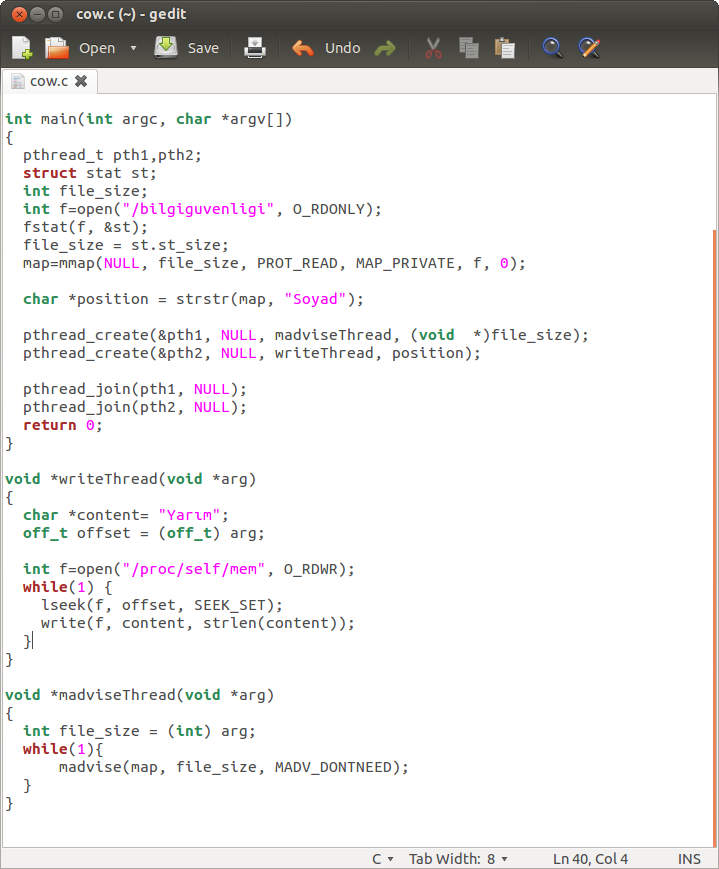
\includegraphics[scale=0.30]{cow-code.png}
        \caption{Uygulama İşlemleri}
    \end{figure}

    Uygulama ilk önce kök dizinde bulunan \textbf{/bilgiguvenligi} adlı dosyayı okumaktadır. Değiştirilecek kısım main bloğunda strstr fonksiyonuyla bulunmakta ve ardından iki thread işlemi çalıştırılmaktadır. Çalıştırılan bu threadlar writeThread() ve madviseThread() fonksiyonlarını çağırmaktadır.

    \textbf{madviseThread()} : Buradaki fonksiyon hafıza üzerinden dosyaya erişim sağlamakta ve eşleştiğinde writeThread fonksiyonuyla eşleşen alana ilgili veri yazılmaktadır.[2]

    \textbf{writeThread()} :  Buradaki fonksiyon dosya içerisinde bulunan alana hafıza üzerinden erişim yaparak veriyi değiştirmektedir.

    Programı çalıştırdıktan sonra belirtilen dosyayı okumuş ve \textbf{Soyad} yazan kelimeyi \textbf{Yarım} olarak değiştirmiştir.
    \begin{figure}[htbp]
        \centering
        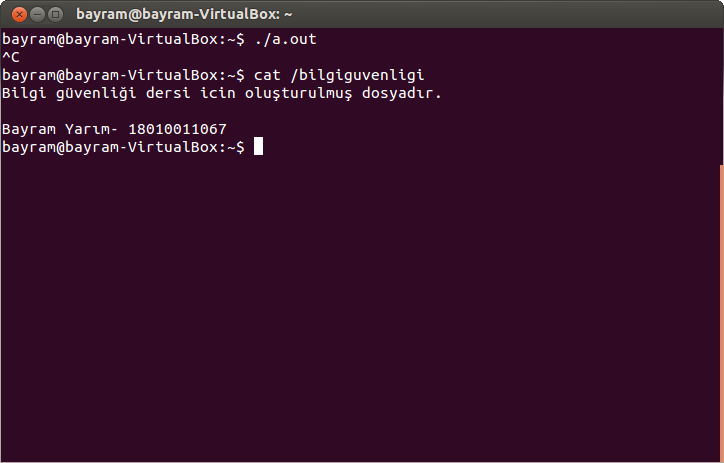
\includegraphics[scale=0.28]{process-out.png}
        \caption{Uygulama Sonucu}
    \end{figure}

    SeedLabs üzerindeki bu örnek uygulamayı yaptıktan sonra asıl görev olan normal kullnıcıyı root kullanıcısına çevirme işlemini yapmaya başladım. Öncelikle sistem de istenildiği gibi \textbf{charlie} adında bir kullanıcı tanımladım ve gerekli bilgilerini girdim. Şekilde görüldüğü üzere sistem üzerinde "charlie" adında bir normal kullanıcı oluşturuldu.

    \begin{figure}[htbp]
        \centering
        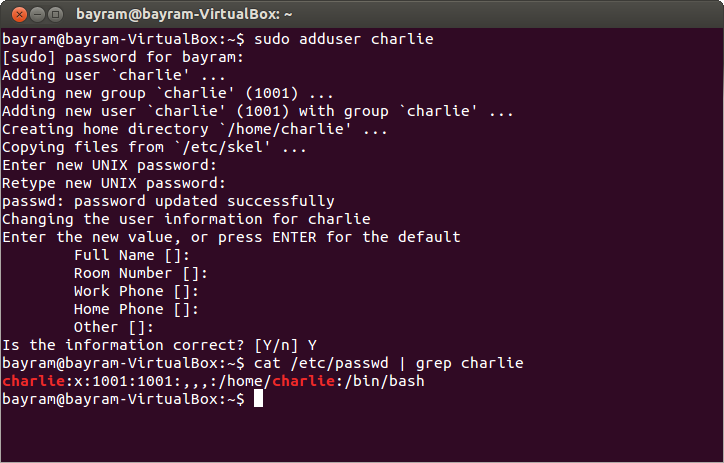
\includegraphics[scale=0.28]{add-user-charlie.png}
        \caption{Normal kullanıcı tanımlama}
    \end{figure}
    Şekil-5 de görüldüğü üzere "charlie" kullanıcısının id numarası 1001'dir. Root kullanıcı numarası ise 0'dır. Kullanıcı id=0 olduğu takdirde kullanıcı kök dizine erişebilen root olarak yetkilendirilmiş olacaktır.

    Kullanıcı tanımından sonra \textbf{"su charlie"} komutuyla charlie kullanıcısına geçiş yaptım ve derlemiş olduğum programı çalıştırdım. Program sistemde o an da aktif kullanıcıyı \textbf{/etc/passwd} içerisinden bulup kullanıcıya \textbf{uid=0} yaparak root yetkisi vermektedir. 
    \begin{figure}[htbp]
        \centering
        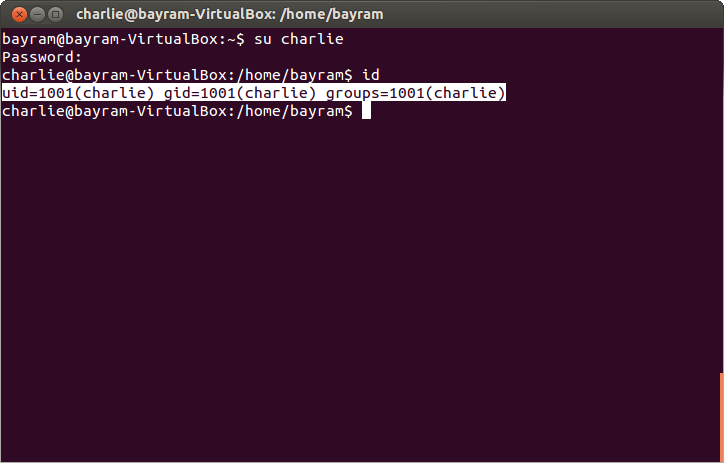
\includegraphics[scale=0.28]{change-user-charlie.png}
        \caption{Kullanıcı Değiştirme}
    \end{figure}
    Uygulama maksimum 10sn içerisinde aktif olan charlie kullanıcısını sistemde buldu ve Dirty COW açığından yararlanarak kullanıcıyı normal kullanıcı modundan root moduna çevirmiştir. Programı durdurup kullanıcı uid komutuyla sorguladığımda kullanıcı yetkisinin root modunda olduğu gözükmektedir.
    \begin{figure}[htbp]
        \centering
        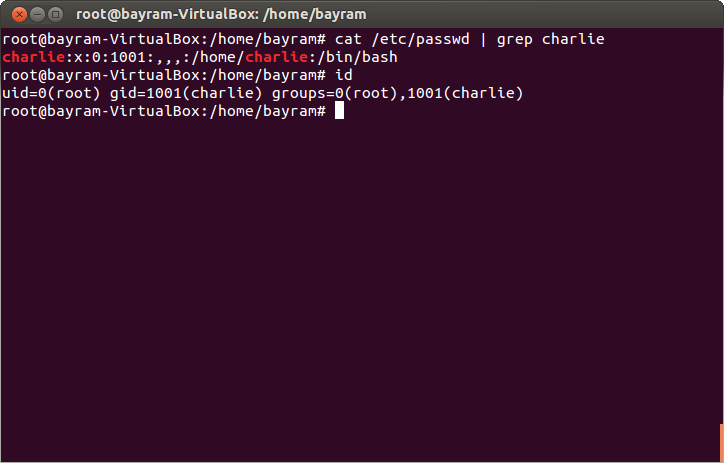
\includegraphics[scale=0.28]{root-charlie.png}
        \caption{Charlie kullanıcısının root modu}
    \end{figure}

    Görüldüğü üzere DirtyCOW güvenlik açığının normal kullanıcıya root yetkisi verdirerek sisteme ne denli zarar vereceğini açıkça ortaya koymaktadır.

\section{Bulgular (Findings)}
    Dirty COW güvenlik açığı, root yetkisi olmayan bir yerel kullanıcının, standart izin mekanizmalarını atlayarak dosyaları değiştirmesine izin verir. Saldırgan, normal bir kullanıcı olarak sistem üzerinde kontrol sahibi olduktan sonra, bir Linux sisteminin tam kontrolünü ele geçirmek için bu güvenlik açığını kullanan bir istismar kullanabilir, kötü amaçlı yazılım yükleyebilir veya verileri çalabilir.

    Bu güvenlik açığı web sunucularını da zarar vermektedir. Araştırmalarda web sunucuların büyük çoğunluğunu linux tabanlı işletim sistemleri oluşturmaktadır. Linux sunucular \%68 ile ilk sırada yer almaktadır. Geri kalanı Windows ve diğer sunucular oluşturmaktadır.

    \begin{figure}[htbp]
        \centering
        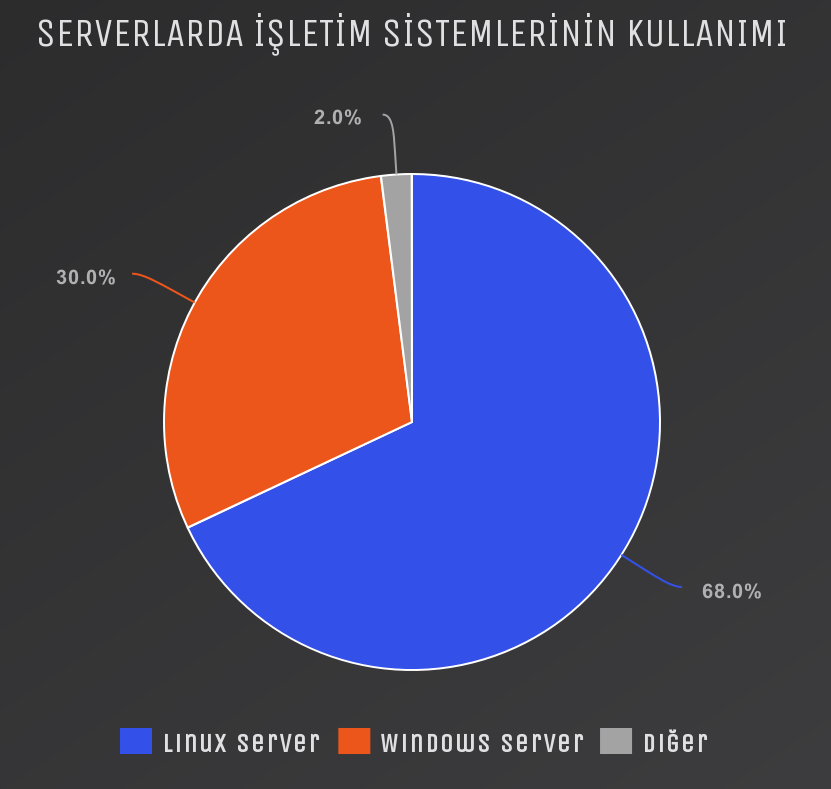
\includegraphics[scale=0.40]{server-grafik.png}
        \caption{Serverlerda İşletim Sistemlerinin Kullanımı}
    \end{figure}

    Linux sunucuların oluşturduğu bu yüzdelik dilimde bir çoğu güncel olmadığı için \%65 lik kısımda güvenlik açıkları halen bulunmaktadır.

    \begin{figure}[htbp]
        \centering
        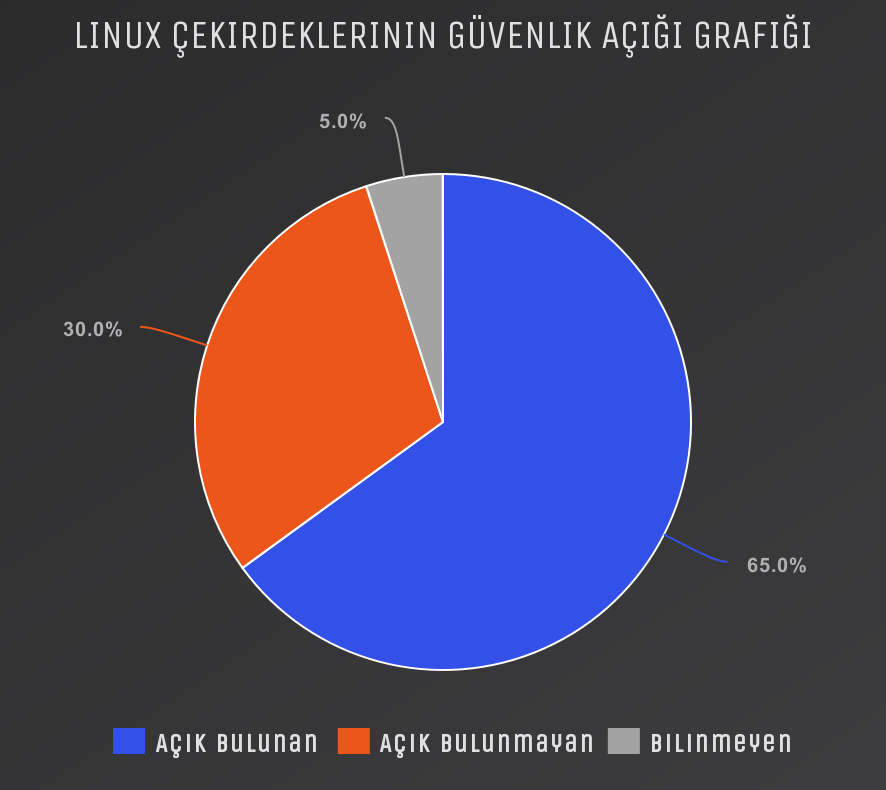
\includegraphics[scale=0.40]{linux-grafik.png}
        %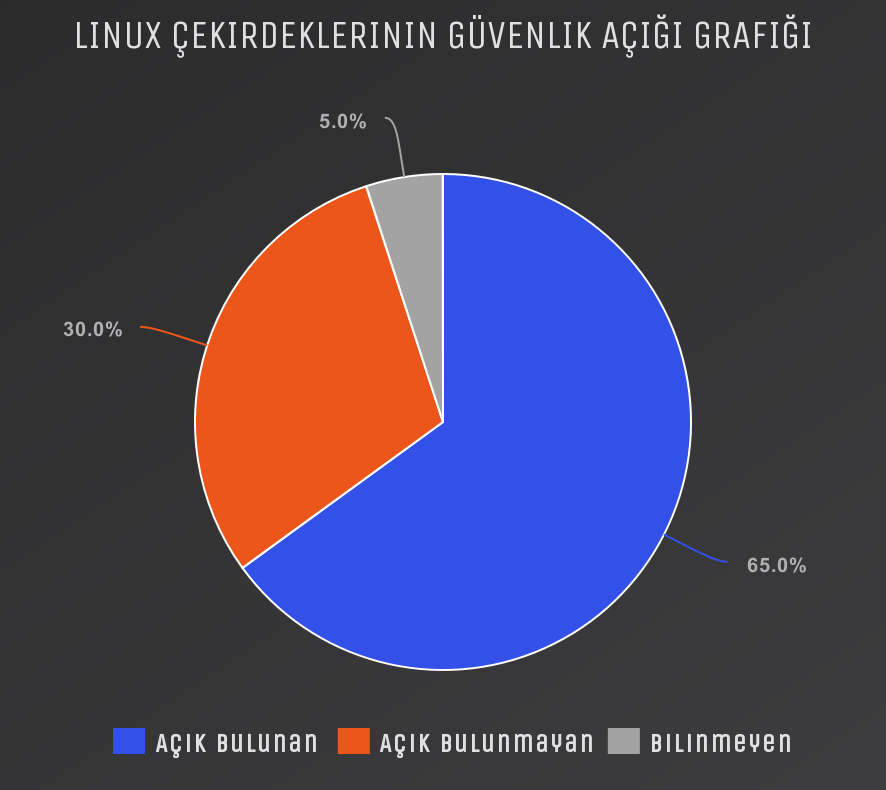
\includegraphics{linux-grafik.png}
        \caption{Linux Çekirdeklerinin Güvenlik Açığı Grafiği}
    \end{figure}

    Dirty COW ile ilgili bir başka durumda, Antivirüs veya herhangi bir güvenlik yazılımı tarafından tespit edilmesinin neredeyse imkansız olması ve istismar edildikten sonra yapılan eylemlere dair hiçbir kanıt kalmamasıdır. Bu açığın en büyük riski, cihazda root düzeyinde erişimin yanı sıra kod yürütme yeteneğinin bulunmasıdır.

    Dirty COW güvenlik açığının bir çok yapı üzerinde uygulaması vardır. Bu uygulamalar github üzerinde oluşturulan bir repoda toparlanmıştır.[4] Uygulamanın youtube videosunu izlemek için linki takip edebilirsiniz.[5]

\section{Sonuç (Conclusion)}
    Yapılan çalışma kodlarıyla salt-okunur dosyaya erişim sağlandı ve hafıza üzerinden dosya içeriği değiştirildi. Yapılan bu işlem linux tarafında tüm salt okunur dosyalara erişebileceğini, yetkisiz kişilere root yetkisi verileceğini göstermiştir. Bunun yanı sıra hafıza üzerinden bir çok verinin değiştirilebileceğini ortaya koymuştur.

    Bu açık ile kernel versiyonu 2.6.22 - 4.8.3 arasında olan tüm linux tabanlı işletim sistemlerinde/cihazlarda uygulanabilir. Kernel versiyonu bu arada bulunan tüm cihazlar güncellenmelidir. 2017 yılında bu güvenlik açığı tamamen kapatılmıştır.
    Güvenlik açığının tüm dökümanlarına ve yapılan çalışmalarına belirtilen web sayfasından erişim sağlayabilirsiniz.[6]

\section{Kaynakça (References)}
\begin{thebibliography}{00}
    \bibitem{b1} https://www.hackread.com/dirty-cow-the-most-linux-bug/
    \bibitem{b2} https://man7.org/linux/man-pages/man2/madvise.2.html
    \bibitem{b3} https://en.wikipedia.org/wiki/Dirty\_COW
    \bibitem{b4} https://github.com/dirtycow/dirtycow.github.io/wiki/PoCs
    \bibitem{b5} https://www.youtube.com/watch?v=kEsshExn7aE\&ab\_channel=LiveOverflow
    \bibitem{b6} https://dirtycow.ninja/
    
\end{thebibliography}

\end{sloppypar}
\end{document}